\chapter*{Method}

\section{Method}
This chapter will describe how the research is executed and which elements that is used. All Hardware, software and processes used will be described to increase the repeatability and validity of the research. The research can be divided into three, lab environment design and tests, traffic capturing and traffic analysis.

\subsection{Tests}
This section will describe the different tests and why they are relevant to the research. Attributes, settings and how the tests are performed will in detailed be described to ensure that all the tests and number of tests are performed the same way.

\subsection{Traffic capturing}
Smart home devices often generates network traffic continuous, as robot vacuum cleaners are cloud based they need to establish and keep alive a secure tunnel where commando and control can be executed. This section will describe how the captures are done and extracted to the location where the packet captures will be analysed. 

\subsection{Traffic Analysis}
To ensure that the research will produce the best contribution to the field of information security. Several different analysis tools will be used, but the main focus will be to use the best satiable machine learning algorithm for this purpose. The Traffic analysis section of this method will include the selection of there methods and, ect    

\section{Smart Home Environment}
To be able to perform passive eavesdropping on a robot vacuum cleaner there have to be set up a lab environment which is able to act similar as a normal smart home environment and allow the traffic and events to be controlled. This parts include the selection of smart home environment, it also includes the selection of devices to use such as robot vacuum cleaner, sniffing hardware and software as well as network design to allow capturing of traffic is the different phases in smart home communication. 

\subsection{Apartment}
The smart home environment will be set up in an apartment in Oslo at Majorstuen, it is 85 m2 where 10 kvm is bathrooms with a height difference on 15 cm. There are two living rooms with a kitchen in between, two bed rooms and an entrance. It is located in the 4th floor of a brick building which have a 5th floor as well, the apartment is therefore surrounded by other apartments. This apartment is chosen because the author of this thesis lives here and it will therefore be a representative live smart home environment.  

\subsection{Robot vacuum cleaner}
Some text

\subsubsection{Robot vacuum selection}
Because of limited resources and time, the selection of equipment needs to be done before acquiring anything. The vacuum will need several smart home features so that the different features can be identified in the network traffic analysis. The purpose of this research is to identify how much private information which can be gathered as well as how complex these types of sniffing attack will have to be. Selecting a vacuum cleaner with more smart home features will potentially reveal more sensitive private information.

IoT devices can use several different network protocols and technology to communicate with other devices. We distinguish between Datalink layer (layer 2), Network layer (layer 3), session layer (layer 4) and Application layer (layer 5). Each of these layers can reveal different information about the session, devices and data which is sent. The Data Link Layer protocol IEEE 802.11 (Wi-Fi) it is the most widespread infrastructure in smart homes \cite{robotsel1}. Wi-fi will therefore be the preferred data link layer protocol, this to ensure the most relevant result \cite{robotsel2}\cite{robotsel3}. The selection of IEEE 802.11 will result in more common Internet routing protocols which supports the principle.

To enable the best user experience possible more and more IoT devices comes with dedicated application for command, control, statistics, and integration. Such applications add new smart home features to devices which often result in more data transfers between the device and the cartelized controller. The application architecture is dependent on the vendor, but a common design is a client-server architecture, where both the vacuum cleaner and mobile application is acting as clients \cite{robotsel4}. This may include sensitive private information transferred between the devices.

Other master students in my study group will focus on the information security aspects of smart home integrated with “home assistant” smart home application. If the robot vacuum cleaner can be integrated in this application as well this could benefit the hole master project group. \cite{robotsel7}

A robot vacuum cleaner will have to navigate around the smart home to be able to clean sufficiently. This navigation is handled differently, form the basic to more advanced navigation. Some of the more advances navigation systems uses laser or camera to navigate and map the environment. \cite{robotsel5} \cite{robotsel6} This type of mapping could generate some interesting information for the research. 

\subsubsection{Network design}
To represent the general smart home in common homes the research used the existing network infrastructure in the apartment and added some components to be able to better isolate the traffic from the robot vacuum cleaner. The different elements are show in figre \ref{fig:HLD}, further each device will be described. 

\begin{figure}[!ht]
    \centering
    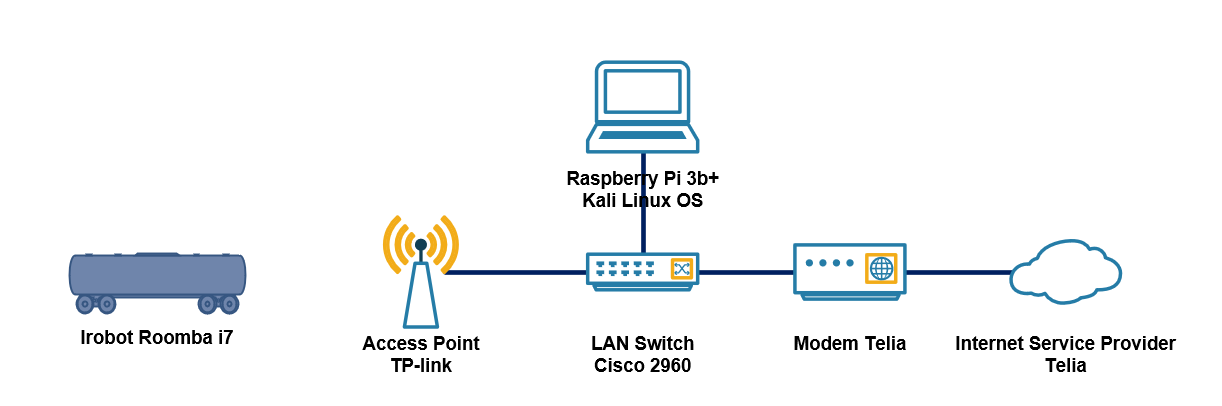
\includegraphics[width=10cm]{figures/HLD.png}
    \caption{Network High Level Design}
    \label{fig:HLD}
\end{figure}

\begin{itemize}
    \item \textbf{Device:} Raspberry Pi 3b+
    \item \textbf{Software:} Kali ARM \cite{kalidownload}, updated 27.09.2022
    \item \textbf{Configuration:}
    \begin{enumerate}
        \item Image downloaded to an external computer and written to the micro SD-card with the application balenaEtcher \cite{balenaetcherdownload}.
        \item Patching done 19.12.2022 with the command "sudo apt update \&\& sudo apt upgrade"
    \end{enumerate}
    \item \textbf{Connected items:}
    \begin{enumerate}
        \item Micro SD card \cite{microsdcard}
        \item TL-WN722N USB WiFi Adapter \cite{tp-link}
    \end{enumerate}
\end{itemize}

\section{Test cases}
Each test Case consists of a detailed test description, which enables the tests and results to be reproduced as identical as possible. It will also state how many times the test was done during the research. The standby traffic test is performed over 14 consecutive days, and all other tests are done 20 times. The number of days and tests are decided based on the available time frame for this master thesis. Equipment selection process, design and configuration process and test phase is time consuming and 20 is therefore chosen as the overall test number. 

\subsection{Baseline-traffic}
Baseline test have the function to represent the traffic flow generated by the robot vacuum cleaner installed in the smart home environment with out any event triggering. For this test the robot vacuum cleaner is installed in the chosen smart home environment described in "smart home environment chapter". Before the test was conducted the robot was operational for more then 60 days, and more then 10 cleaning jobs done. This to ensure that is is in operational mode.

\begin{itemize}
    \item \textbf{Description:} Conduct packet sniffing for both wireless and cabled traffic generated over a number consecutive days. Capture data is stored in two separate files. The Robot vacuum cleaner is connected to power and Internet the entire time period.
    \item \textbf{Number of tests:} 14 consecutive days
\end{itemize}

\subsection{Triggered cleaning}
Triggered cleaning is an event started trough the IRobot application with the use of "start cleaning". The test is done when the mobile application receives a notification that the cleaning is done. If the robot vacuum need to return to base to recharge, empty bin or get stuck something in the brushes, actions will be done to enable the robot to continue cleaning. 
\begin{itemize}
    \item \textbf{Description:} Start cleaning through the Irobot application, with the use of start cleaning. Capture is started 10 minutes before cleaning is scheduled and stopped 30 minutes after the cleaning is finished. 
    \item \textbf{Number of tests:} 20
\end{itemize}

\subsection{Empty bin} The bin needs to be removed from the vacuum cleaner to be emptied. This will make the vacuum cleaner in a state where is cannot start cleaning, and the application will display information about the situation. 

\begin{itemize}
    \item \textbf{Description:}Start packet capturing 5 minutes before the bin is removed. Remove the bin, wait 5 minutes and then insert the bin once more. Stop capturing 5 minutes after the bin is inserted
    \item \textbf{Number of tests:}20
\end{itemize}

\subsection{Open mobile application}
Mobile application will be able to access information about the robot vacuum cleaner. This might generate pull requests from the Irobot cloud towards the vacuum cleaner to get the needed information to display. If the user changes attribute in the application this needs to be communicated with the vacuum cleaner. 
\begin{itemize}
    \item \textbf{Description:} Start packet capturing 5 minutes before opening the application on the smart phone. Open the application, change a "room name" and one "room separation line", then wait until the application have been open for 5 minutes, then close the application. Stop packet capturing after additionally 5 minutes. 
    \item \textbf{Number of tests:}20
\end{itemize}



\section{Methods in relates work}
Through some one the papers review in the related work section they used to capture live traffic from the smart devices.In this section the different methods in \cite{lindaeavesdropping} \cite{eavsIoT} \cite{Neato}, will be discussed and elements that could be used in this research will be identified and justified. 


\begin{itemize}
    \item \textbf{Description:}
    \item \textbf{Number of tests:}20
\end{itemize}